\section{GENERAL GEOLOGY (The 1st Floor Room)}
\label{chap:general-geology}

\section{Geological evolution}
\label{sec:geological-evolution}

The Earth has experienced a vast and dynamic history of about 4 billion years. This journey is divided into major geological eons and eras, each defined by important events such as the formation of the crust, shifts in the atmosphere, the rise of life, and tectonic movements. These processes become clearer when explored alongside physical specimens and visual displays, such as those presented at the Ho Chi Minh City Geological Museum.

\subsection{Precambrian: 4 billion to 570 million years ago (~600 million years)}
\label{subsec:precambrian}

\subsubsection{Archean Eon (4.0–2.6 billion years ago)}
\label{subsubsec:archean}

It is one of the earliest chapters in Earth's history, when the crust stabilized, continents and oceans first formed, and simple life such as stromatolite-building cyanobacteria appeared, slowly altering the planet's atmosphere.

In Vietnam, Archean rocks are found in the Kon Tum geoblock, mainly within the Kan Nack Group. These 3,000-meter-thick metamorphic rocks show complex changes, from granulite facies to amphibolite and greenschist facies, revealing the intense geological processes that shaped the ancient Earth.

\begin{figure}[H]
  \centering
  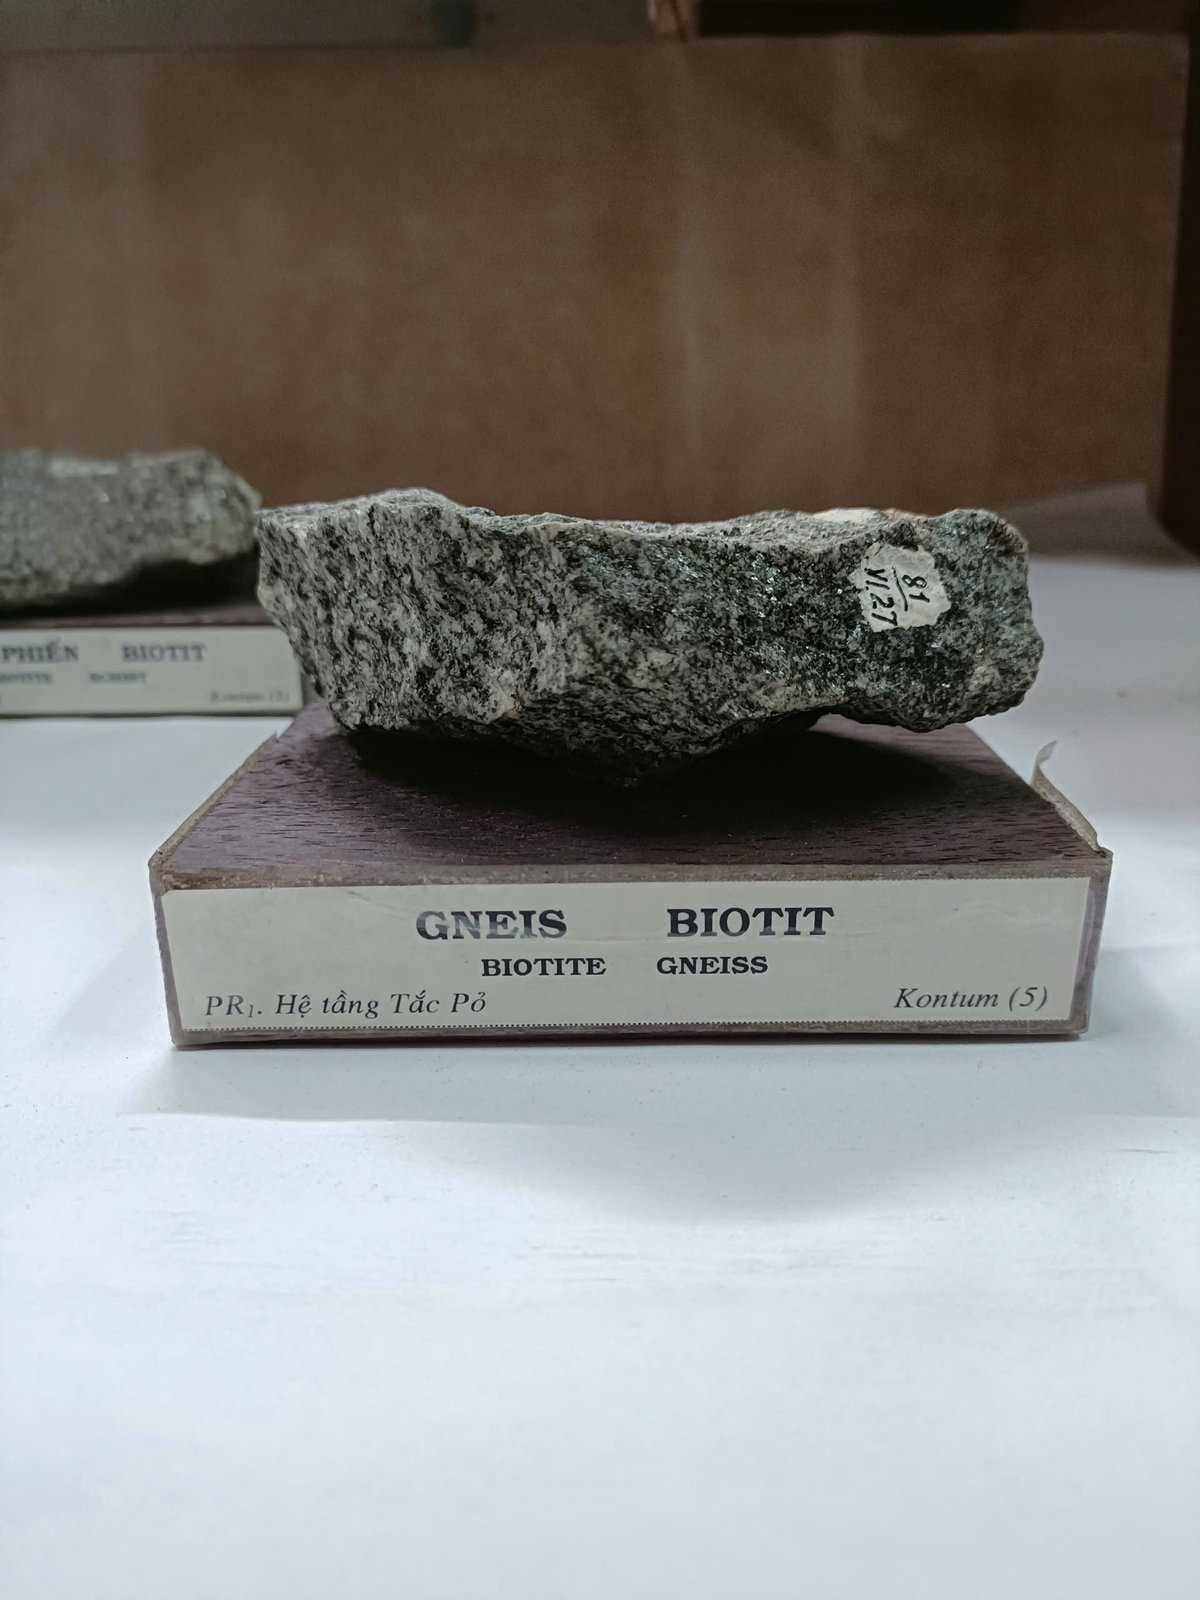
\includegraphics[max width=0.8\linewidth]{graphics/figure_02.jpg}
  \caption{Sample of rock in Archean Eon}
  \label{fig:archean-rock}
\end{figure}

\subsubsection{Proterozoic Eon (2.6 billion to 570 million years ago)}
\label{subsubsec:proterozoic}

It saw the Great Oxidation Event, global ice ages called "Snowball Earth," and the rise of the first multicellular life, including the Ediacaran biota. These changes prepared the planet for the Cambrian explosion of life.

In Vietnam, rocks from the Proterozoic are found in areas like Red River, Fansipan, Chay River, Ma River, Phu Hoat, and Kon Tum. These include crystalline and metamorphic rocks as well as younger layers that lead into the Cambrian period. Some of these rocks contain fossils of tiny early life forms.

\begin{figure}[H]
  \centering
  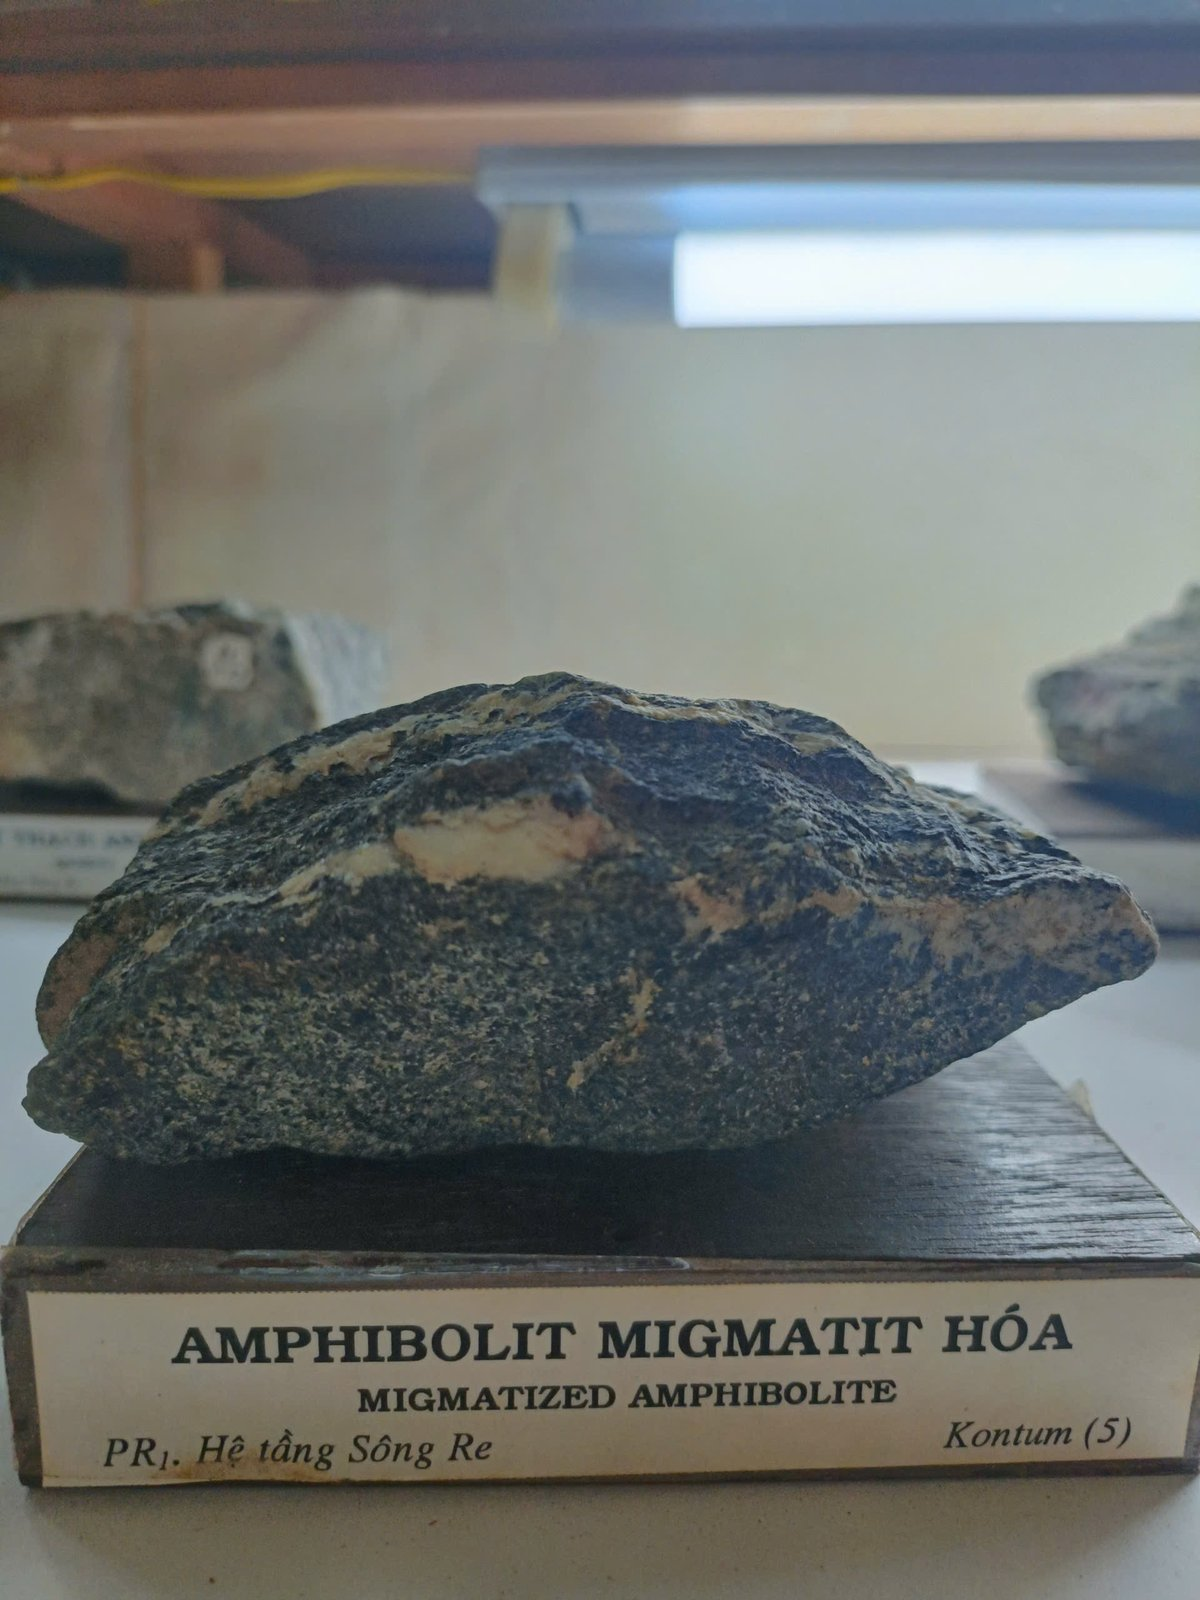
\includegraphics[max width=0.8\linewidth]{graphics/figure_03.jpg}
  \caption{Sample of rock in Proterozoic Eon}
  \label{fig:proterozoic-rock}
\end{figure}

\subsection{Paleozoic Era (570 million to 250 million years ago)}
\label{subsec:paleozoic}

It is divided into six periods: Cambrian, Ordovician, Silurian, Devonian, Carboniferous, and Permian. During this time, ocean life expanded rapidly with animals like trilobites, corals, crinoids, brachiopods, graptolites, and cephalopods.

In Vietnam, many rocks from the Paleozoic Era can still be found today. In regions like North Vietnam, Northwest Vietnam, Northeast Vietnam, and Central Vietnam, the rocks are made of limestone and other sediments that contain fossils of trilobites, brachiopods, and corals.

\begin{figure}[H]
  \centering
  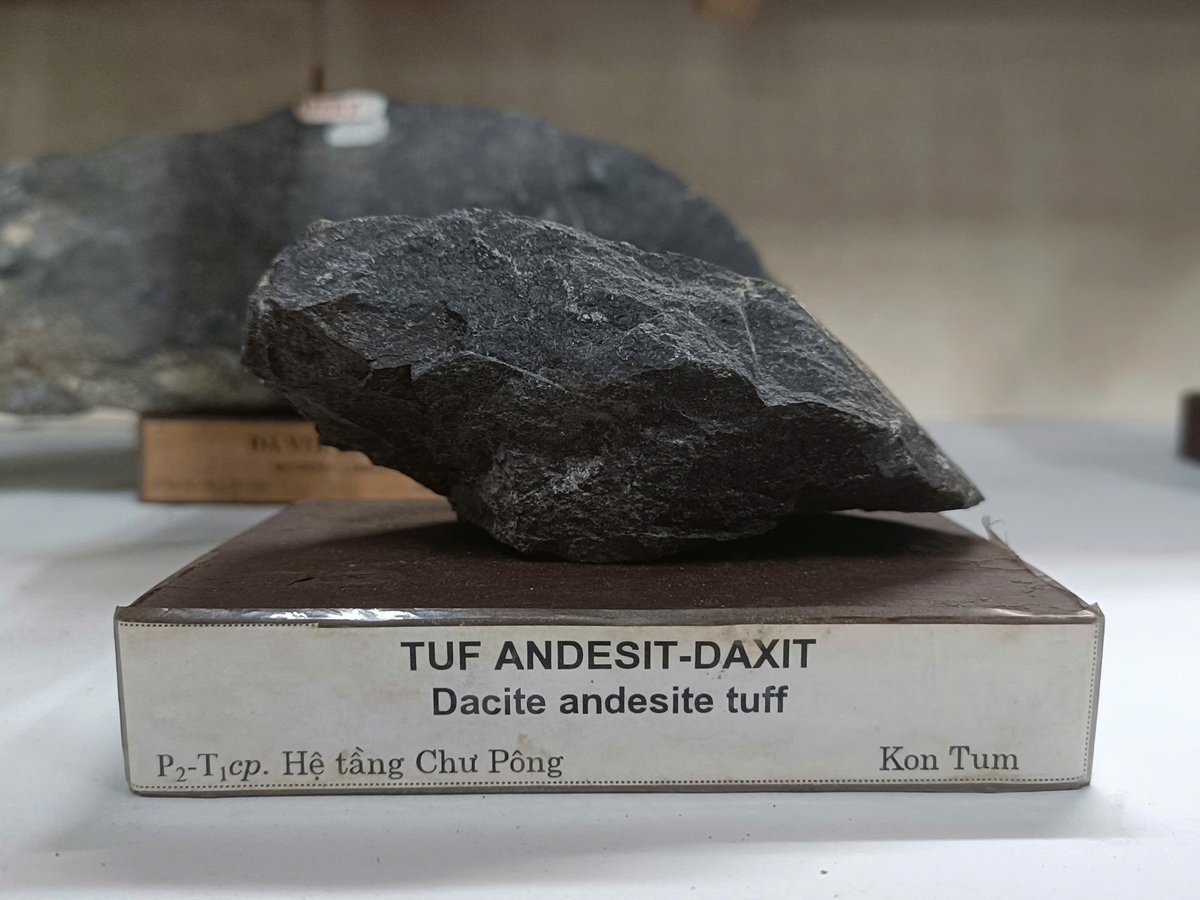
\includegraphics[max width=0.8\linewidth]{graphics/figure_04.jpg}
  \caption{Sample of rock in Paleozoic Era}
  \label{fig:paleozoic-rock}
\end{figure}

\subsection{Mesozoic Era (250 million to 64 million years ago)}
\label{subsec:mesozoic}

It is divided into three periods: Triassic, Jurassic, and Cretaceous. This era is famous as the "Age of Reptiles," when dinosaurs, ammonites, and many other creatures lived, along with early plants and marine animals like bivalves and brachiopods.

In Vietnam, Mesozoic rocks are found in places such as An Chau, Da River, Hien River, and Southwest. Triassic rocks here contain fossils of ammonites, gastropods, plants, and bivalves. Later, during the Jurassic and Cretaceous, red continental rocks and coal-bearing formations appeared, especially in the North, while volcanic rocks developed in areas like Tam Lang and Tu Le. These layers preserve fossils that show how both land and sea environments changed during this era.

\begin{figure}[H]
  \centering
  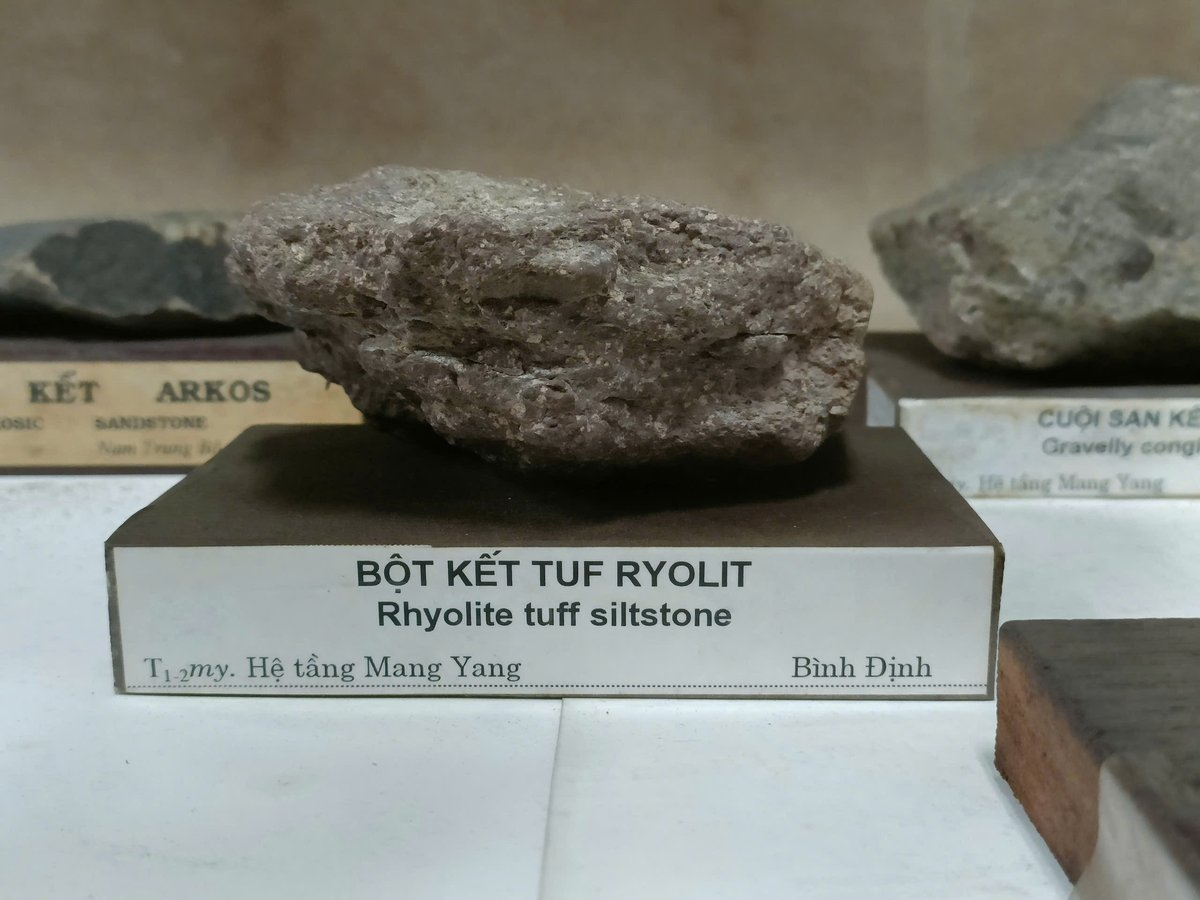
\includegraphics[max width=0.8\linewidth]{graphics/figure_05.jpg}
  \caption{Sample of rock in Mesozoic Era}
  \label{fig:mesozoic-rock}
\end{figure}

\subsection{Cenozoic Era (64 million years ago to present)}
\label{subsec:cenozoic}

It is divided into three periods: Paleogene (70–25 million years ago), Neogene (25–1.8 million years ago), and the Quaternary (1.8 million years ago to today). This era is marked by great diversification of life, with many plants, mollusks, diatoms, ostracods, foraminifers, and vertebrates flourishing.

In Vietnam, Cenozoic rocks are found in regions such as Northwest (Pu Tra, Nam Bay), South Central Coast, and coastal basins. Paleogene rocks are rare, but Neogene sediments are widespread, often containing coal, kaolin, bentonite, and diatomite. These layers also include volcanic rocks, lagoon and delta deposits, and shallow marine formations, preserving fossils that show the rich environments of Vietnam during this era.

\begin{figure}[H]
  \centering
  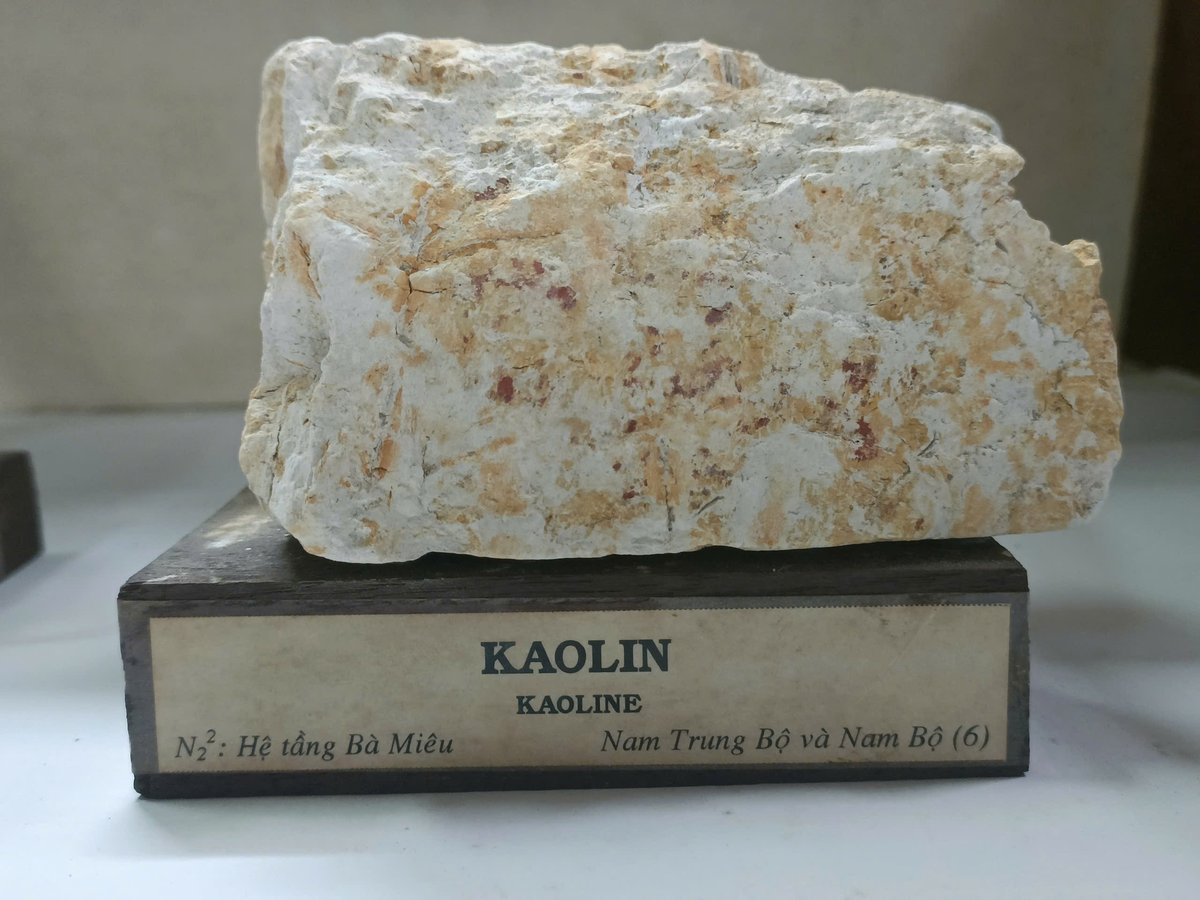
\includegraphics[max width=0.8\linewidth]{graphics/figure_06.jpg}
  \caption{Sample of rock in Cenozoic Era}
  \label{fig:cenozoic-rock}
\end{figure}

\section{Geological Process}
\label{sec:geological-process}

Geological processes are natural forces that continuously shape and alter both the Earth's surface and its interior. At the Ho Chi Minh City Geological Museum, visitors were introduced to six key geological processes through rock samples, models, and diagrams. These processes—ranging from extraterrestrial impacts to deep-earth activity and surface transformations—drive the creation, modification, and recycling of Earth's materials. The museum's exhibits illustrated how each process contributes to the formation of various rocks and landforms, highlighting the dynamic and interconnected system of the geological cycle.

\subsection{Cosmic process}
\label{subsec:cosmic-process}

The cosmic process refers to extraterrestrial impacts, mainly from meteorites, that influenced Earth's early development. These collisions produced craters, altered surface rocks, and introduced vital elements such as iron, nickel, and platinum, which became fundamental to the planet's crust and core. Studied through meteorite discoveries worldwide, this process underscores Earth's origins in space.

\subsection{Tectonic process}
\label{subsec:tectonic-process}

Tectonic processes refer to the movement of Earth's lithospheric plates, which drive major geological events such as earthquakes, volcanic eruptions, mountain building, and continental drift. At the museum, this concept was demonstrated using global tectonic maps and a 3D model of plate boundaries, highlighting where and how the plates interact. The exhibit illustrated three main boundary types:

\begin{itemize}
  \item Divergent boundaries, where plates separate and new crust is created.
  \item Convergent boundaries, where plates collide, causing subduction and mountain formation.
  \item Transform boundaries, where plates slide past one another, triggering earthquakes.
\end{itemize}

Through these visuals, the display showed how plate interactions fuel geological activity and continually reshape Earth's surface.

\subsection{Magmatic process}
\label{subsec:magmatic-process}

Magmatic processes are responsible for forming igneous rocks when magma cools and solidifies. The appearance and composition of these rocks depend on how quickly and where the cooling takes place. This explains why igneous rocks can look very different from one another, even though they all come from the same basic process.

In the museum, igneous rocks were divided into two main groups. Extrusive rocks, such as basalt and andesite, form when lava erupts onto the Earth's surface and cools very quickly. Because the cooling is so fast, crystals don't have time to grow, resulting in a fine-grained texture. On the other hand, intrusive rocks, like granite and diorite, form deep underground where magma cools slowly over long periods of time. This slow cooling allows large crystals to develop, giving the rocks a coarse, grainy texture.

\begin{figure}[H]
  \centering
  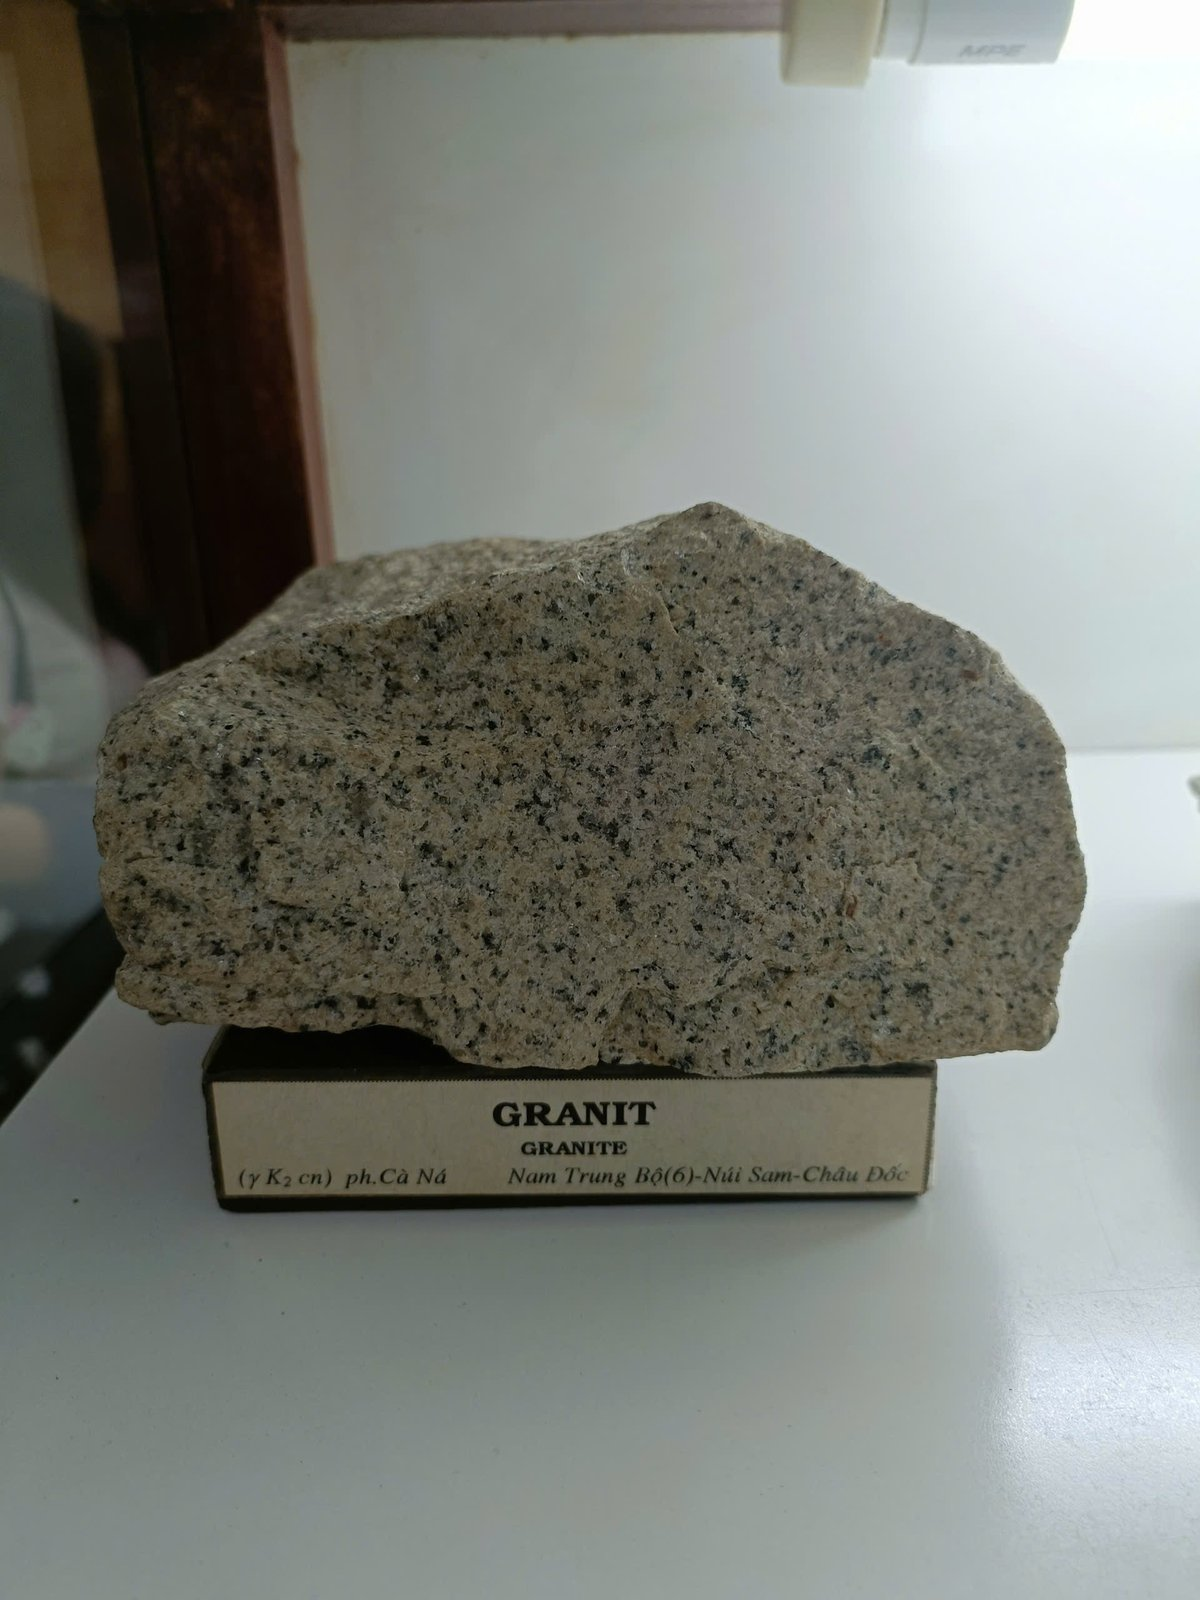
\includegraphics[max width=0.8\linewidth]{graphics/figure_07.jpg}
  \caption{Sample of intrusive igneous rock}
  \label{fig:intrusive-igneous}
\end{figure}

\subsection{Metamorphic process}
\label{subsec:metamorphic-process}

Metamorphism happens when existing rocks undergo high heat, strong pressure, or interaction with reactive fluids, leading them to change into new rock types. At the museum, specimens like schist, gneiss, slate, quartzite, and marble were displayed, each representing different metamorphic environments.

One highlighted example was marble, which develops from limestone through contact metamorphism. The exhibit also included diagrams of metamorphic facies and processes, illustrating how different conditions drive these rock transformations.

\begin{figure}[H]
  \centering
  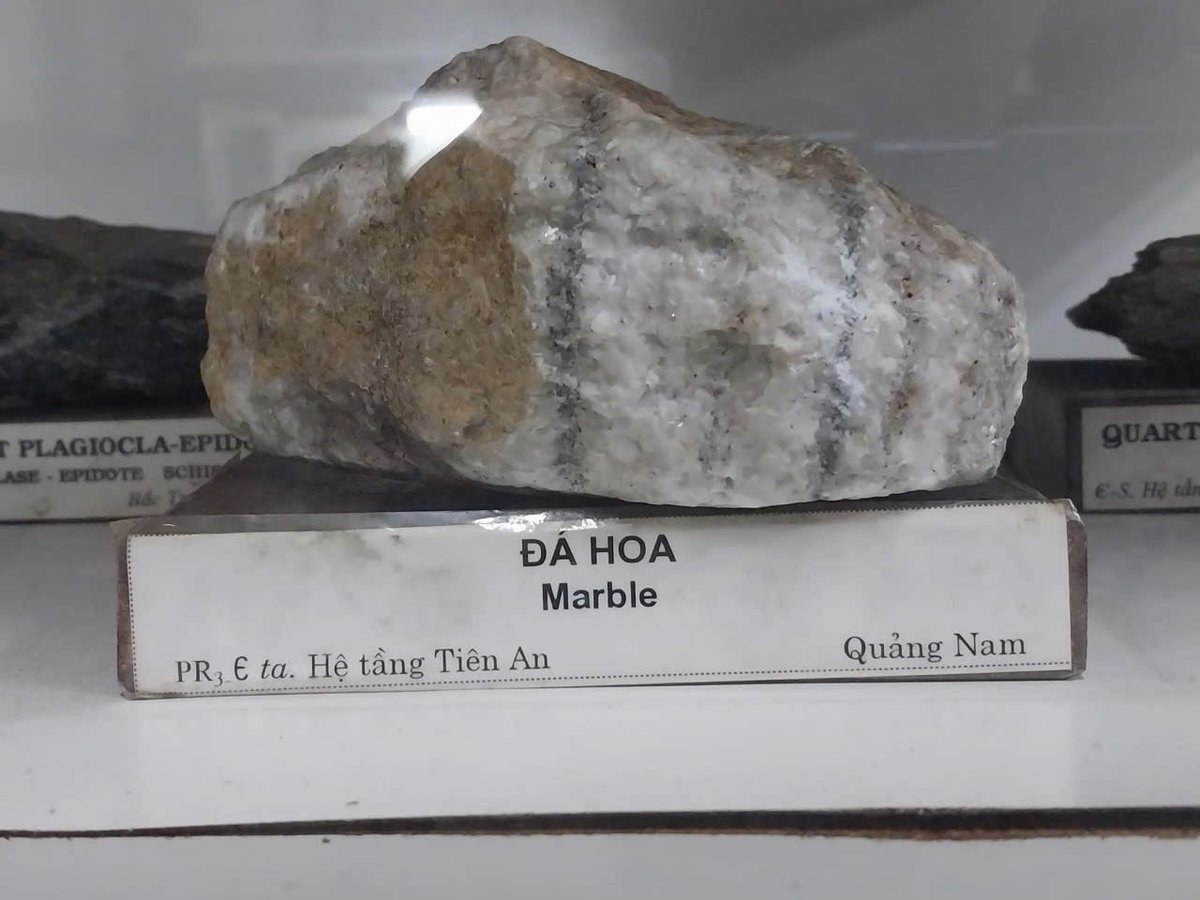
\includegraphics[max width=0.8\linewidth]{graphics/figure_08.jpg}
  \caption{Sample of Marble}
  \label{fig:marble}
\end{figure}

\subsection{Sedimentary process}
\label{subsec:sedimentary-process}

Sedimentary processes occur when materials from older rocks or biological sources are gathered, compressed, and cemented together, resulting in sedimentary rocks that typically show layered structures.

\begin{itemize}
  \item Mechanical sedimentation produces rocks such as sandstone and conglomerate, created from the physical breakdown and accumulation of rock fragments.
  \item Chemical sedimentation is seen in rocks like limestone, which forms when minerals precipitate from water-rich solutions.
\end{itemize}

\begin{figure}[H]
  \centering
  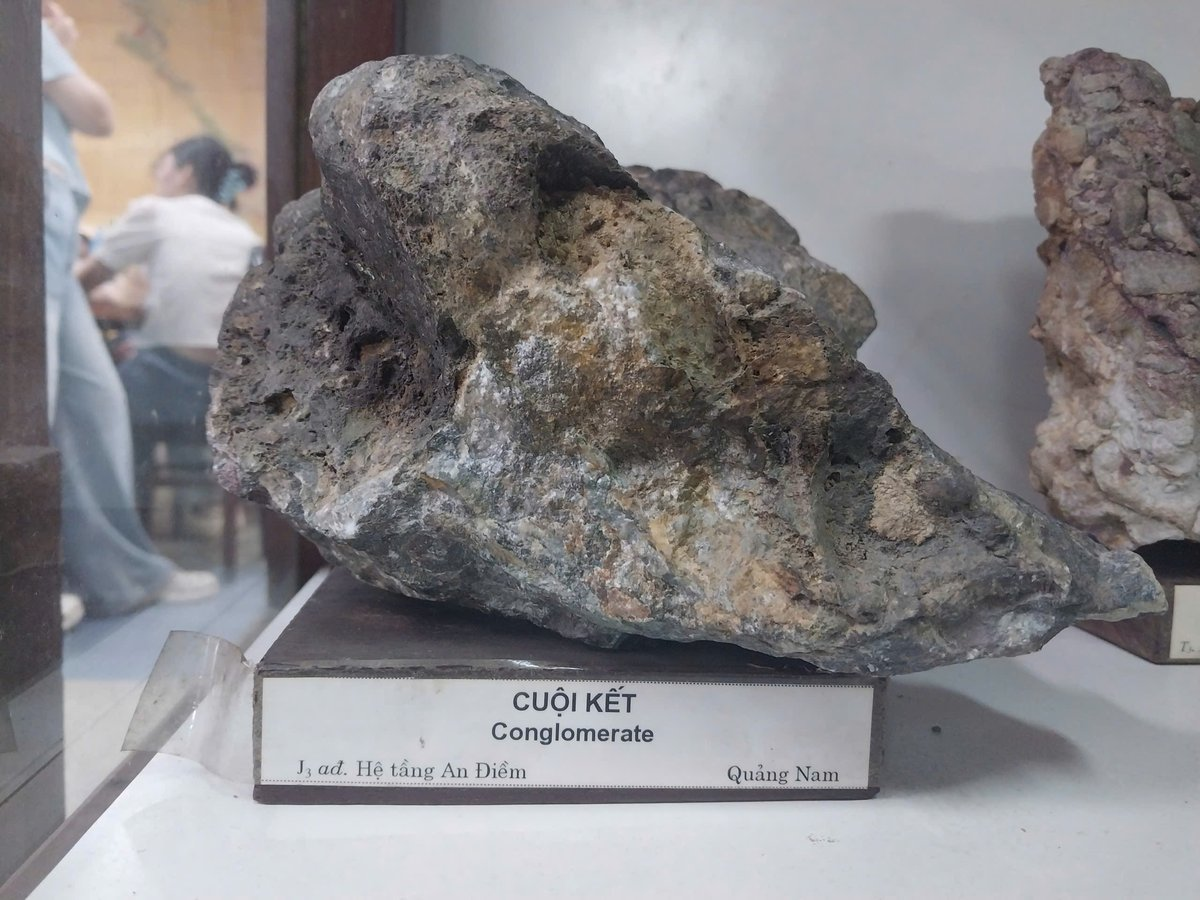
\includegraphics[max width=0.8\linewidth]{graphics/figure_09.jpg}
  \caption{Sample of Mechanical sedimentation rock}
  \label{fig:mechanical-sedimentation}
\end{figure}

\subsection{Weathering process}
\label{subsec:weathering-process}

Weathering is the natural process that breaks down rocks at Earth's surface through the effects of wind, rainfall, temperature changes, and chemical reactions. At the museum, this was demonstrated with diagrams and rock samples that showed how rocks are altered by different types of weathering.

Examples included mechanical weathering, such as rock fragmentation and exfoliation, and chemical weathering, like the oxidation of iron on rock surfaces. These displays highlighted weathering's important role in the rock cycle, as it produces loose sediments that can later compact and cement to form sedimentary rocks.

\begin{figure}[H]
  \centering
  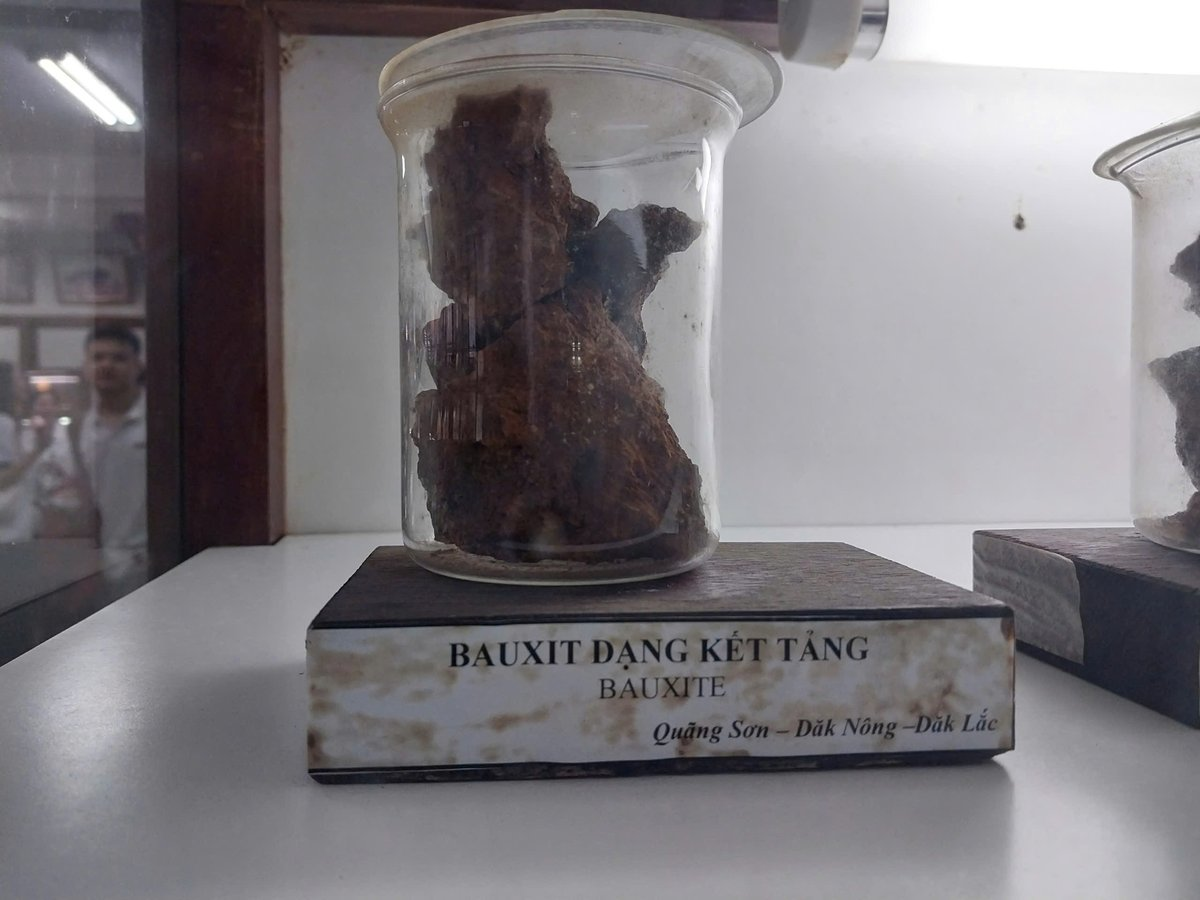
\includegraphics[max width=0.8\linewidth]{graphics/figure_10.jpg}
\caption{Sample of Bauxite}
\label{fig:bauxite}
\end{figure}